\documentclass[twocolumn]{article}
\usepackage[utf8]{inputenc}
\usepackage{graphicx}
\usepackage{textcomp}
\usepackage{fullpage}
\usepackage{float}

\title{Simple CDMA Decoding Project}
\author{Nikita Teplitskiy }

\begin{document}
\maketitle

\section{Introduction}

The submitted project is a successful implementation of a CDMA decoder based on a simplified CDMA implementation. The encoded message was \textit{"The ships hung in the sky in much the same way that bricks don't."} which is a quote from the Hithikers Guide to the Galaxy.

\section{M Sequence Offset Determination}

In order to decode the incoming signal it is essential to locate the offset of the PN sequence with which the signal was originally encoded. In an incorrect offset is selected, the resulting decoded signal will appear as noise and it will be impossible to recover any of the encoded data. Luckily, recovering the PN offset is easy by employing cross correlation between a known PN sequence and the incoming signal. 

\begin{figure}[h]
    \centering
    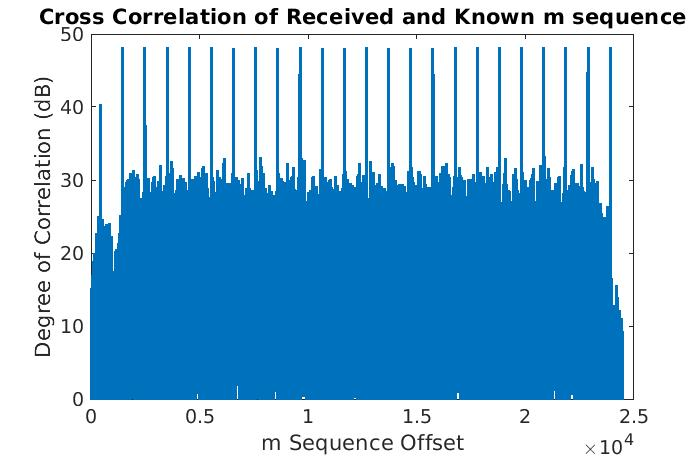
\includegraphics[width=0.45\textwidth]{oldpn.jpg}
    \caption{}
    \label{fig}
\end{figure}

The result is shown in Figure 1 where clearly defined spikes in correlation are visible. These spikes occur whenever the known PN sequence matches up with the PN sequence used to encode the signal. According to the provided instructions, a new PN sequence begins at the start of a frame which occurs once every 255 chips. Since the peaks shown in Figure 1 do not align on frame boundaries, the reference PN sequence is shifted until they do. The result of this is shown in Figure 2.

\begin{figure}[h]
    \centering
    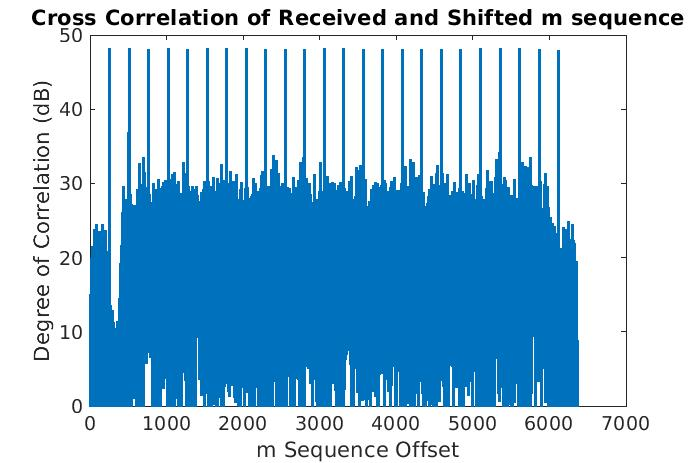
\includegraphics[width=0.45\textwidth]{newpn.jpg}
    \caption{}
    \label{fig}
\end{figure}

\section{Pilot Extraction}

To simplify decoding and detection, CDMA systems include a Pilot Channel made up of a known stream of data. For this assignment, the Pilot Channel constantly transmits the 0th channel from an 8-ary Walsh Code. Since the 0th Walsh Code is always 0, decoding it is trivial. Before that occurs, the PN spreading code must removed from the received signal. This significantly cleans up the signal as shown in figures 3 and 4. After removing the PN sequence, the pilot can be recovered by integrating and normalizing over the extent of the Walsh code. This results in the radially distributed set of clusters shown in Figure 5. 

\begin{figure}[H]
    \centering
    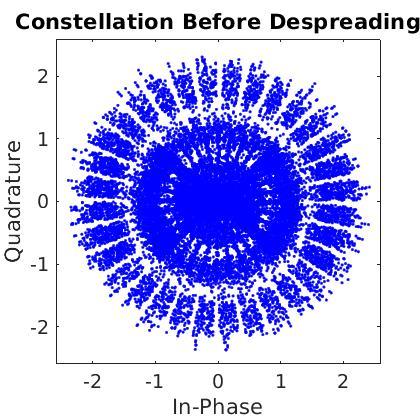
\includegraphics[width=0.35\textwidth]{Uconst.jpg}
    \caption{}
    \label{fig:my_label}
\end{figure}
\begin{figure}[H]
    \centering
    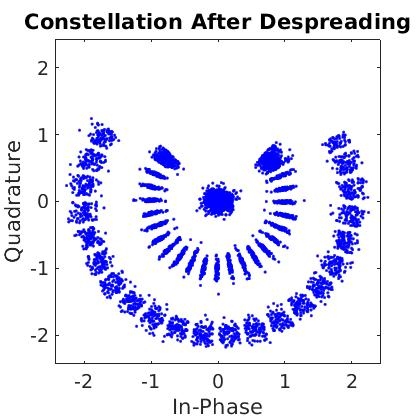
\includegraphics[width=0.35\textwidth]{Sconst.jpg}
    \caption{}
    \label{fig}
\end{figure}
\begin{figure}[H]
    \centering
    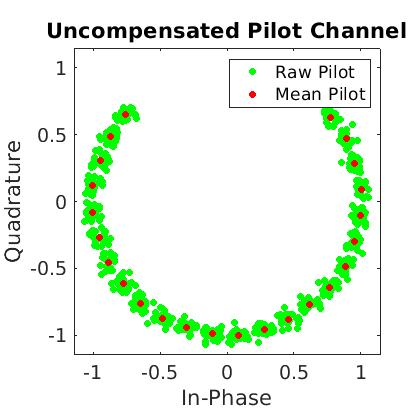
\includegraphics[width=0.35\textwidth]{PilotChan.jpg}
    \caption{}
    \label{fig}
\end{figure}

The radial distribution of the pilot channel reveals that the received signal possesses a small frequency offset that gradually alters the phase of all data in the channel. Since the Pilot Channel is known to always transmit a 1, finding the inverse of the mean Pilot Channel in each frame will correct the frequency offset of the Pilot. Furthermore, the same correction can be applied to the remaining data in the signal. 

\section{Data Recovery}

After applying the frequency compensation from the previous section to the entire signal, the data channel can extracted. This achieved by subtracting the value of the Pilot Channel from the remaining data and multiplying it by the 5th Walsh Code. After integrating and normalizing the result, the signal is thresholded to $\pm 1$ and demodulated. This binary data is then converted into 8-bit ASCII which reveals the hidden message.

\section{Frequency and Phase Recovery}

By using a majestic and powerful algorithm that is too long to be included on this page, a frequency and phase offset of 31 Hz and 0.63 radians was computed. It may also be possible that the phase offset is $0.63 + \pi$, but that would degrade the visual appeal of Figure 6. (I tested a limited number of frequency and phase offsets for performance improvements) 

\begin{figure}[h]
    \centering
    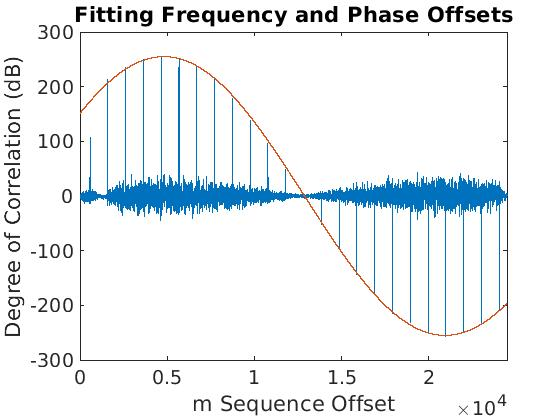
\includegraphics[width=0.45\textwidth]{FPfit.jpg}
    \caption{}
    \label{fig}
\end{figure}

 
\end{document}
 
